\documentclass{report}
\title{Report del dashboard}
\date{26/07/2024}
\author{Pietro Olivetti}

\usepackage{paracol}
\usepackage{Sweave}
\linespread{1.5}

\begin{document}
\Sconcordance{concordance:informe.tex:informe.Rnw:1 16 1 1 10 88 1}


\title{Informe sobre la investigación - Reino Unido: datos sociodemográficos, salud y depresión}

\maketitle





\section{Introducción}

Este informe es parte de un reto relativo al módulo de Visualización de Datos del Masters de Ciencia de Datos Comportamental, de la Universidad de Barcelona. Para definir la investigación, la motivación inventada para la realización del reto ha sido la siguiente: los destinatarios del dashboard serían los stakeholders de una Organización No Gubernamental 
(ONG) británica que procura identificar y atender a personas en situación de vulnerabilidad 
socioeconómica. La exploración de estos datos buscaría comprender el perfil de los individuos que 
presentan mayor riesgo de depresión.  Luego, se trataría de una audiencia que está habituada a datos 
sociodemográficos, pero es la primera vez que buscan más informaciones relativas a la salud de 
los individuos, de forma que podríamos considerar que tienen un nivel de conocimiento 
moderado para interpretar el dashboard. Todos los análisis se realizarán en el entorno de la IDE 
RStudio, conjuntamente con herramientas para la investigación reproducible como  Github, 
Shiny y Markdown. 

\section{Objetivos}

\begin{itemize}
\item El objetivo principal de esta investigación es de explorar como variables de salud impactan en la intensidad de los síntomas de depresión.
\begin{itemize}
\item	Analizar los perfiles sociodemográficos de las personas con niveles más intensos de la variable indicadora de depresión. 
\item	Analizar las diferencias entre los perfiles de personas en vulnerabilidad económica y el resto de la muestra. 
\item	Analizar el impacto del consumo de alcohol y tabaco sobre la variable indicadora de depresión.
\end{itemize}
\end{itemize}

\subsection{Preguntas de la ONG:} 


\textit{¿Hay una diferencia significativa de la prevalencia del síntoma de sentirse deprimido entre las personas que viven en vulnerabilidad económica y las que no viven en esta condición? (Utilizaremos como umbral menos de 380 libras por semana para abarcar todos los perfiles).} 


\begin{itemize}
\item Personas con niveles de ingreso 1 y 2 tienen mucho más probabilidad de presentar niveles de síntoma depresivo más grandes que las personas que tienen otro tipo de ingreso. Vivir en situación de vulnerabilidad económica parece ser un indicador importante dado la discrepancia entre los números indicados en los gráficos.Personas pobres a manifestar niveles de depresión más intensos comparados a toda la muestra. La muestra que manifiesta un nivel moderado o más intenso es de 196 personas (el 16.7\%). De esa sub-muestra, las personas en vulnerabilidad económica representan un 46\% del total.
\end{itemize}

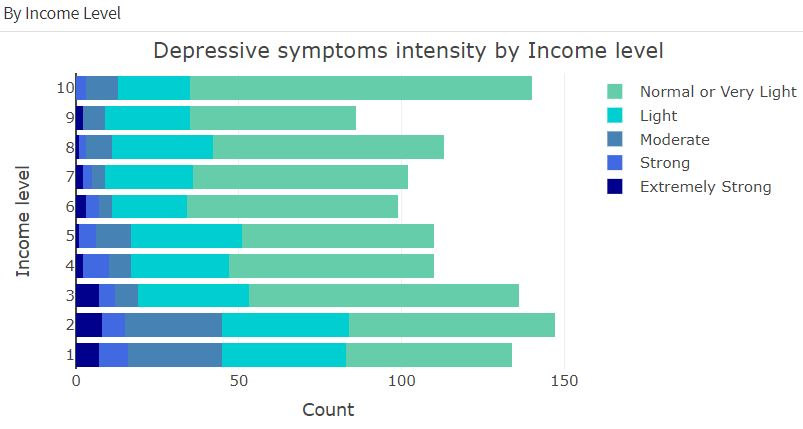
\includegraphics[width=1\textwidth]{dep_by_income.JPG}



\textit{¿Individuos que experimentan problemas de salud tienen mayor probabilidad de 
manifestar el síntoma depresivo? }

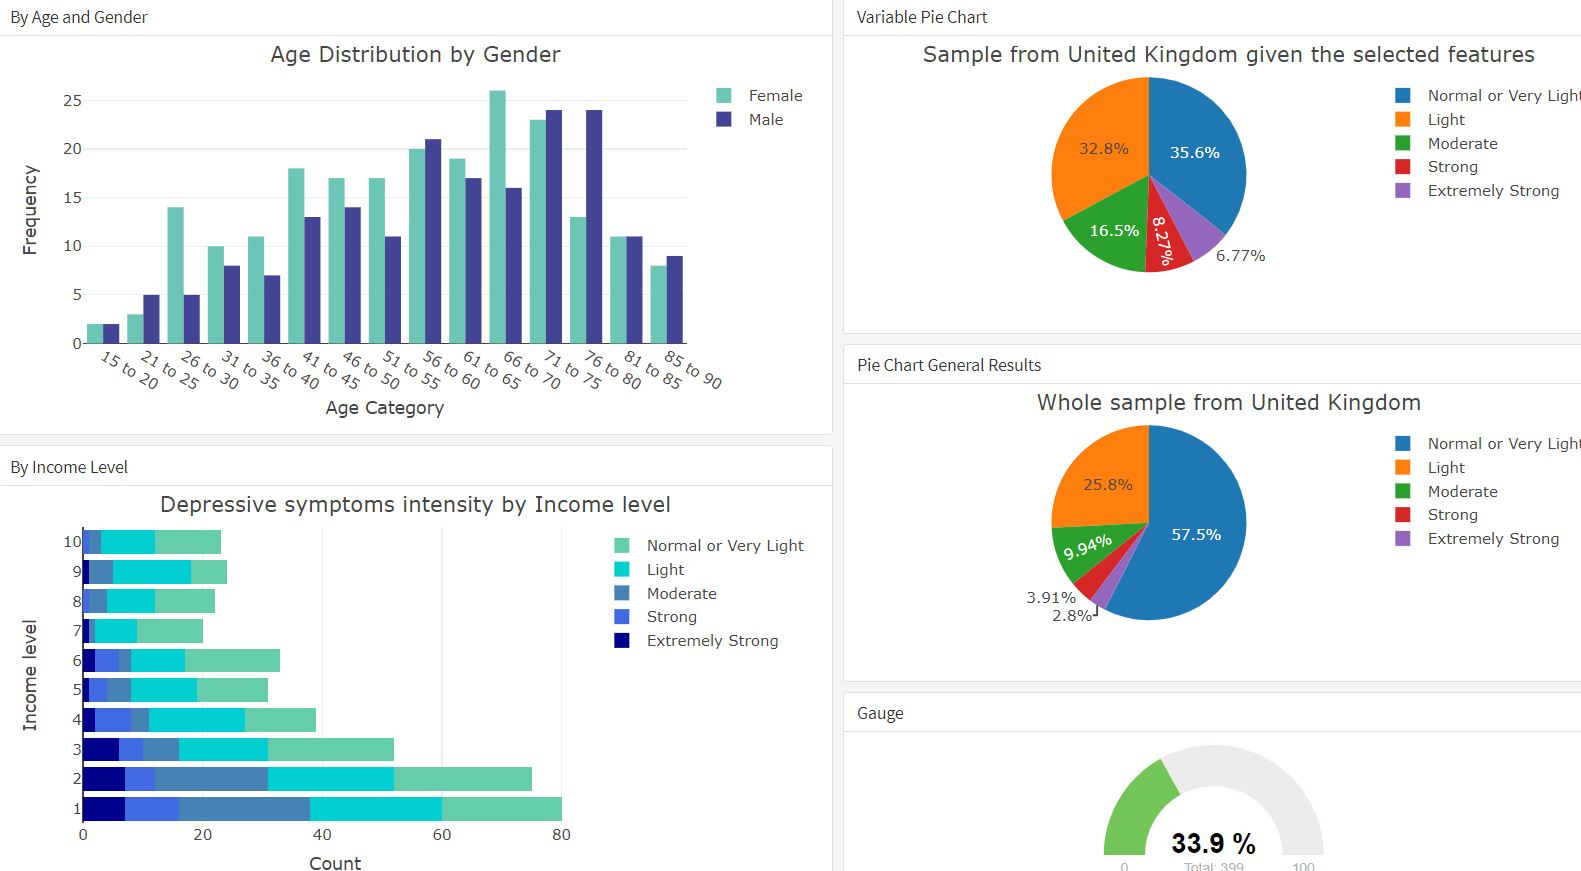
\includegraphics[width=1\textwidth]{dep_hampered.JPG}

\begin{itemize}
\item Personas que tienen enfermedades que impactan la vida diaria son el 34\% de la muestra. El 22.1\% tienen un nivel moderado de molestias mientras que los 11.9\% restantes son muy impactados. Esas dificultades afectan también los síntomas depresivos en relación a los niveles de ingreso. Se nota un acumulo significativo de niveles más intensos de depresión en las categorías más bajas de ingreso. De forma general, personas afectadas por enfermedades que dificultan la vida diaria tienen riesgos más grandes de manifestar síntomas más intensos.
\end{itemize}

\textit{¿Cuál es el impacto de la inaccesibilidad a los servicios de salud en los nivel de síntoma 
depresivo más intensos? }

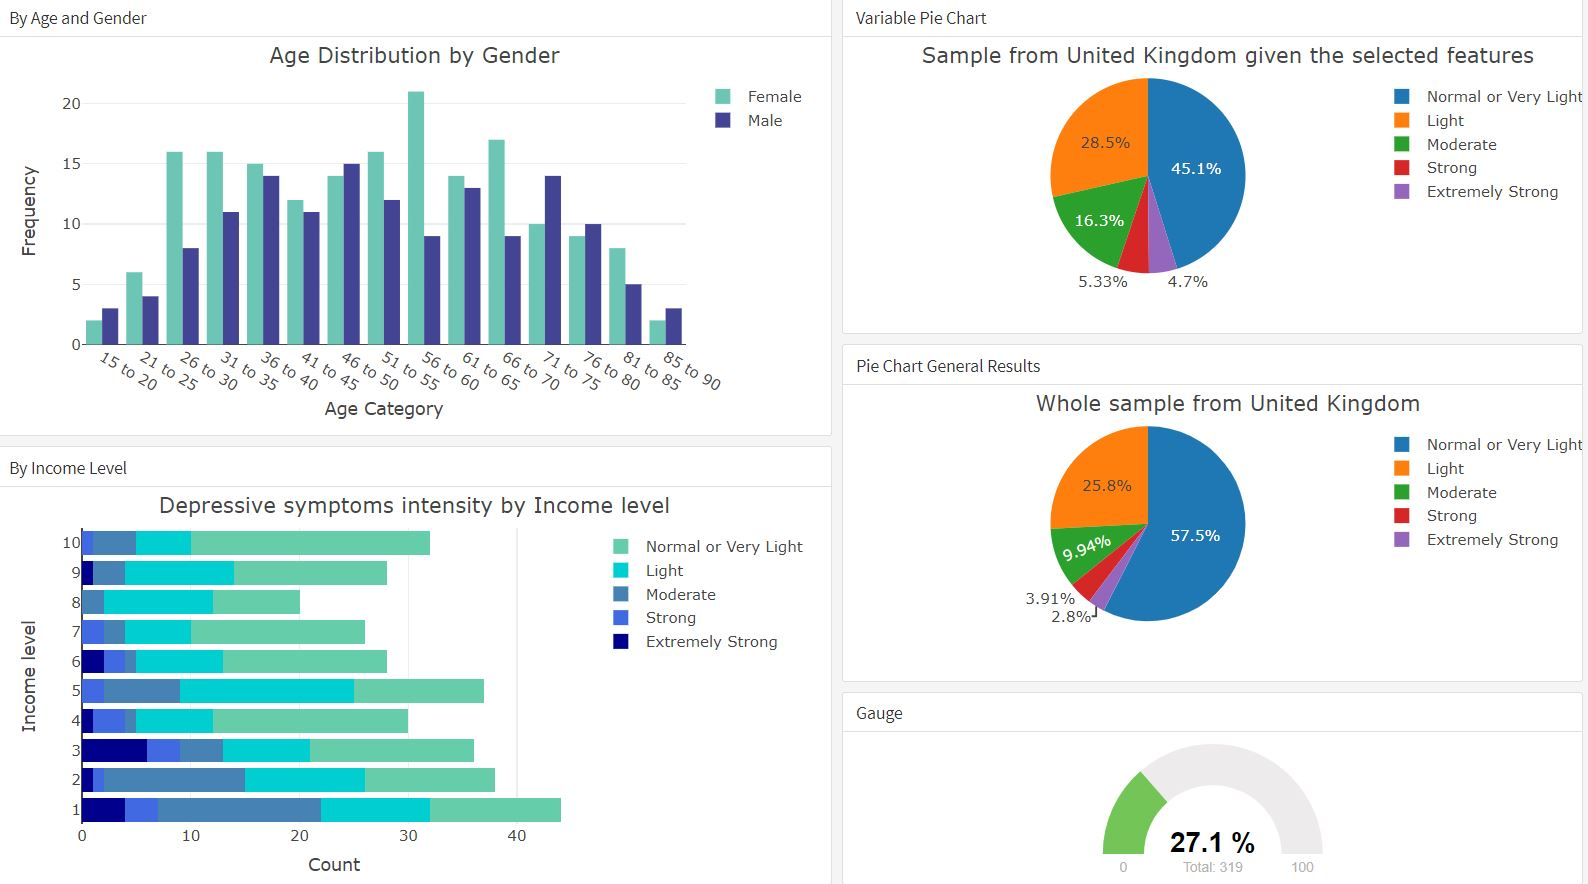
\includegraphics[width=1\textwidth]{dep_no_access.JPG}

\begin{itemize}
\item El 27.1\% de la muestra no logró tener acceso a servicios de salud en los últimos 12 meses. No parece haber una prevalencia pronunciada en relación a género o nivel de ingreso. De forma general parece ser un problema amplio en varios segmentos demográficos de Reino Unido. Sin embargo, como ya hemos visto, es importante resaltar que el síntoma depresivo se manifiesta más intensamente en personas más pobres sin acceso a los servicios de salud.
\end{itemize}

\textit{¿Las variables sociodemográficas de edad y género indican prevalencia del síntoma 
depresivo más intenso (niveles moderado o más intensos)?}

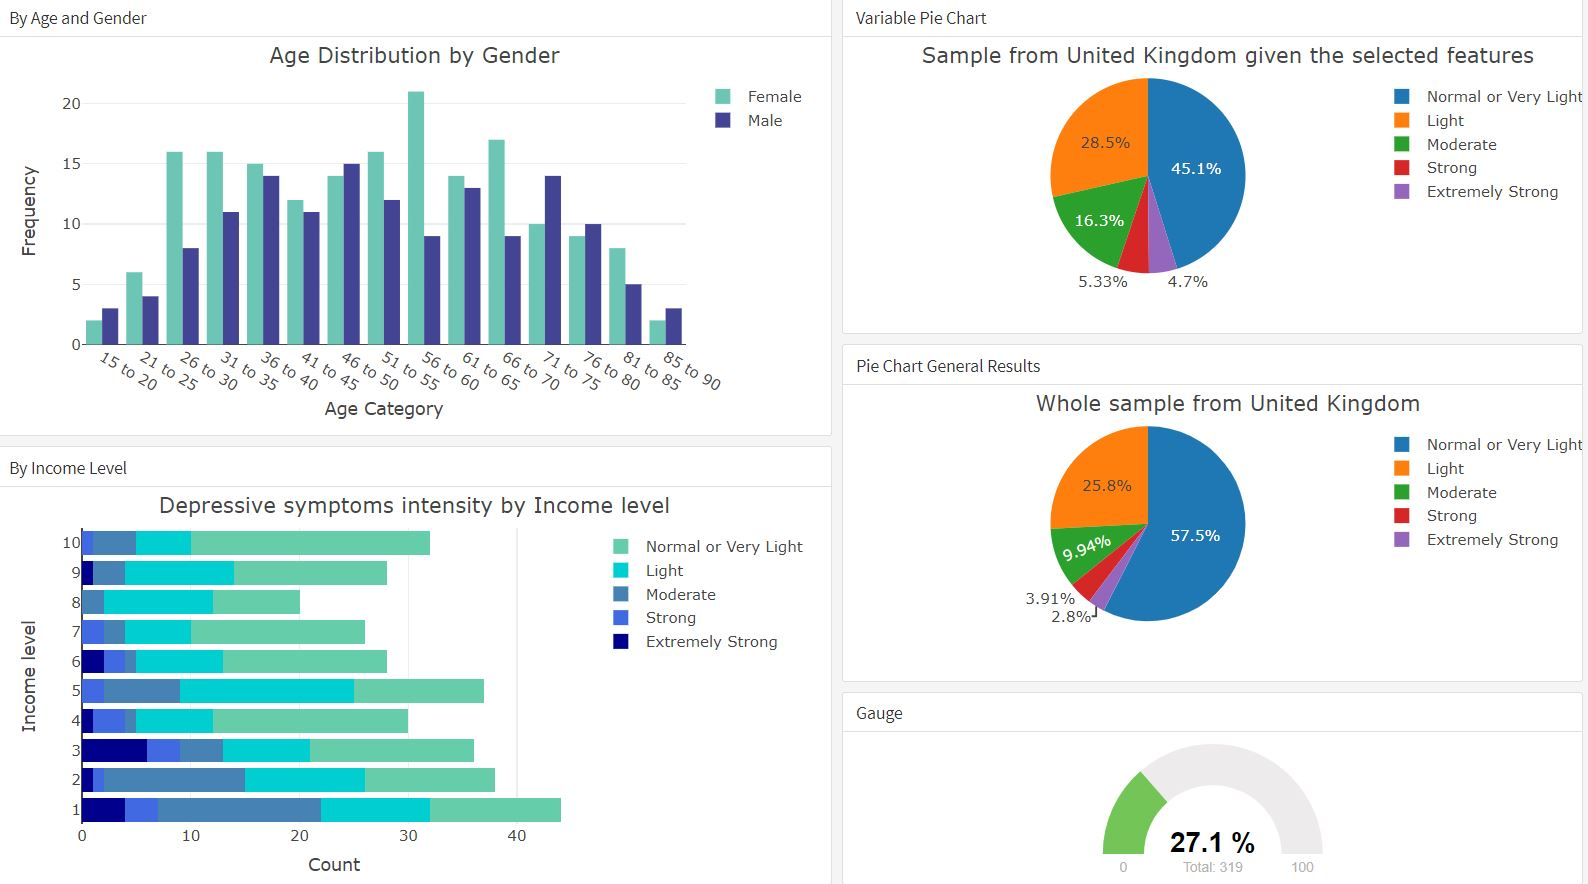
\includegraphics[width=1\textwidth]{dep_no_access.JPG}

\begin{itemize}
\item De forma general, mujeres jóvenes parecen manifestar síntomas más intensos en números más grandes. A partir de los 40 años, las mujeres siguen con números más elevados, pero mucho menos discrepantes en relación a los hombres.
\end{itemize}

\textit{¿Personas que fuman diariamente tienen más probabilidad de manifestar síntomas de depresión?}

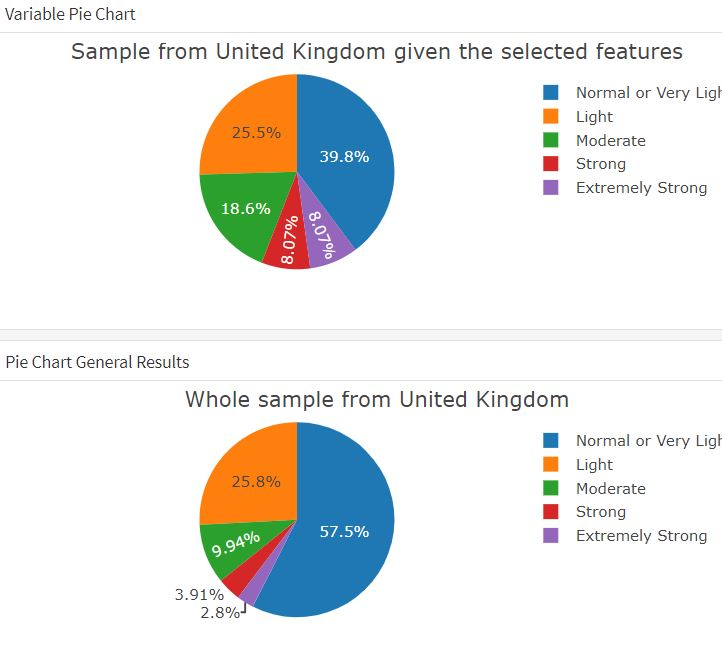
\includegraphics[width=1\textwidth]{daily_cig.JPG}

\begin{itemize}
\item Un 13.7\% de la muestra fuma diariamente. Se puede notar que la proporción de personas que fuman diariamente y que tienen un nivel moderado o superior de síntomas depresivos es el doble en relación al grupo de personas que no fuman o lo hacen raramente. 
\end{itemize}


\textit{¿Personas que beben alcohol varias veces por semana o diariamente tienen más probabilidades de experimentar síntomas depresivos intensos?}

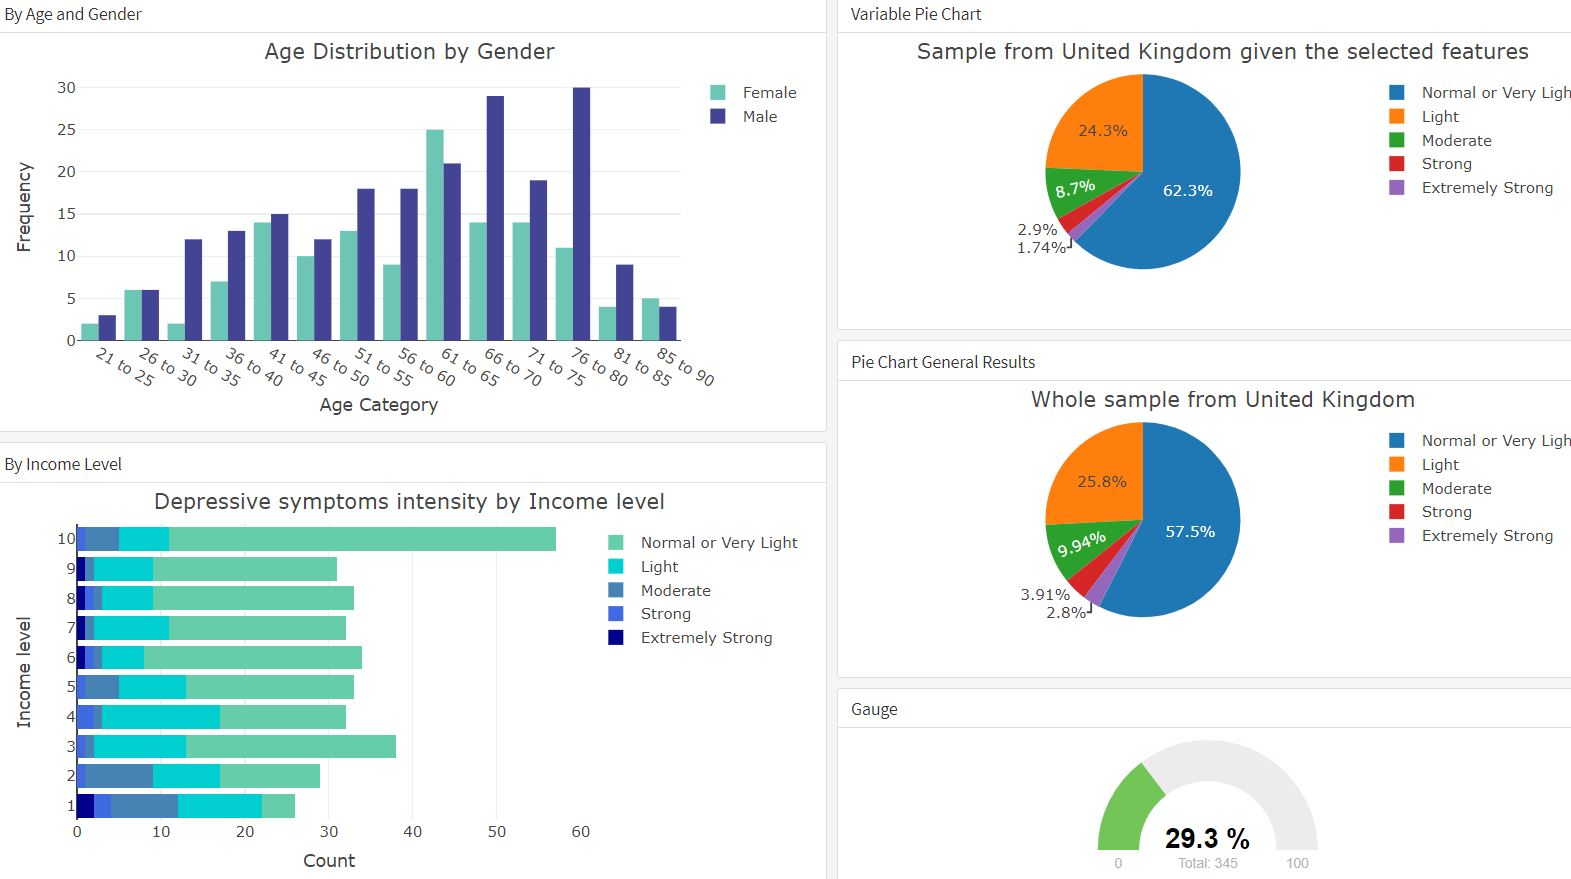
\includegraphics[width=1\textwidth]{dep_alc.JPG}

\begin{itemize}
\item Un 29.3\% de la muestra consume alcohol varios días por semana o todos los días. Curiosamente, el consumo más intenso de alcohol no ha impactado la muestra de forma negativa. Hay más personas que no experimentan síntomas de depresión entre los que consumen alcohol frecuentemente comparado con la muestra general. Sin embargo, la cantidad de personas más pobres con el mismo perfil de consumo presenta síntomas más de mayor intensidad en números más grandes.
\end{itemize}



\end{document}


